As a complement to the inverse dynamics analysis, closed loop simulations were conducted for the wPCC. The simulation results are shown in \autoref{fig:sim_wPCC}. The predicted overshoot angles for the zigzag10/10 are about one degree larger than the experiments as shown in \autoref{fig:overshoots_wPCC}. For the 20/20, the first overshoot is about one degree larger for the polynomial rudder and two degrees larger for the semi-empirical rudder. The corresponding values for the second overshoots are 1.5 and 3 degrees.       

\begin{figure}[h]
     \centering
     \begin{subfigure}[b]{\textwidth}
         \centering
         \includesvg[height=0.3\textheight]{figures/results_wPCC_ID.closed loop zigzag 10_10 port.svg}
        \caption{Simulations wPCC Zigzag10/10 to port.}
        \label{fig:sim_wPCC_10}
     \end{subfigure}
     \vfill
     \begin{subfigure}[b]{\textwidth}
        \centering
        \includesvg[height=0.3\textheight]{figures/results_wPCC_ID.closed loop zigzag 20_20 stbd.svg}
        \caption{Simulations wPCC Zigzag20/20 to starboard.}
        \label{fig:sim_wPCC_20}
     \end{subfigure}
        \caption{Comparison between zigzag tests with wPCC from experiments and simulations with a model equipped with either a polynomial rudder or semi-empirical rudder model.}
        \label{fig:sim_wPCC}
\end{figure}

\begin{figure}[h]
     \centering
     \begin{subfigure}[b]{\textwidth}
         \centering
         \includesvg{figures/results_wPCC_ID.overshoot1.svg}
        \caption{First overshoot angles.}
        \label{fig:overhoots1_wPCC}
     \end{subfigure}
     \vfill
     \begin{subfigure}[b]{\textwidth}
         \centering
         \includesvg{figures/results_wPCC_ID.overshoot2.svg}
        \caption{Second overshoot angles.}
        \label{fig:overhoots2_wPCC}
     \end{subfigure}
     
        \caption{Overshoot angles from the wPCC experiments and simulations.}
        \label{fig:overshoots_wPCC}
\end{figure}

\begin{figure}[h]
    \centering
    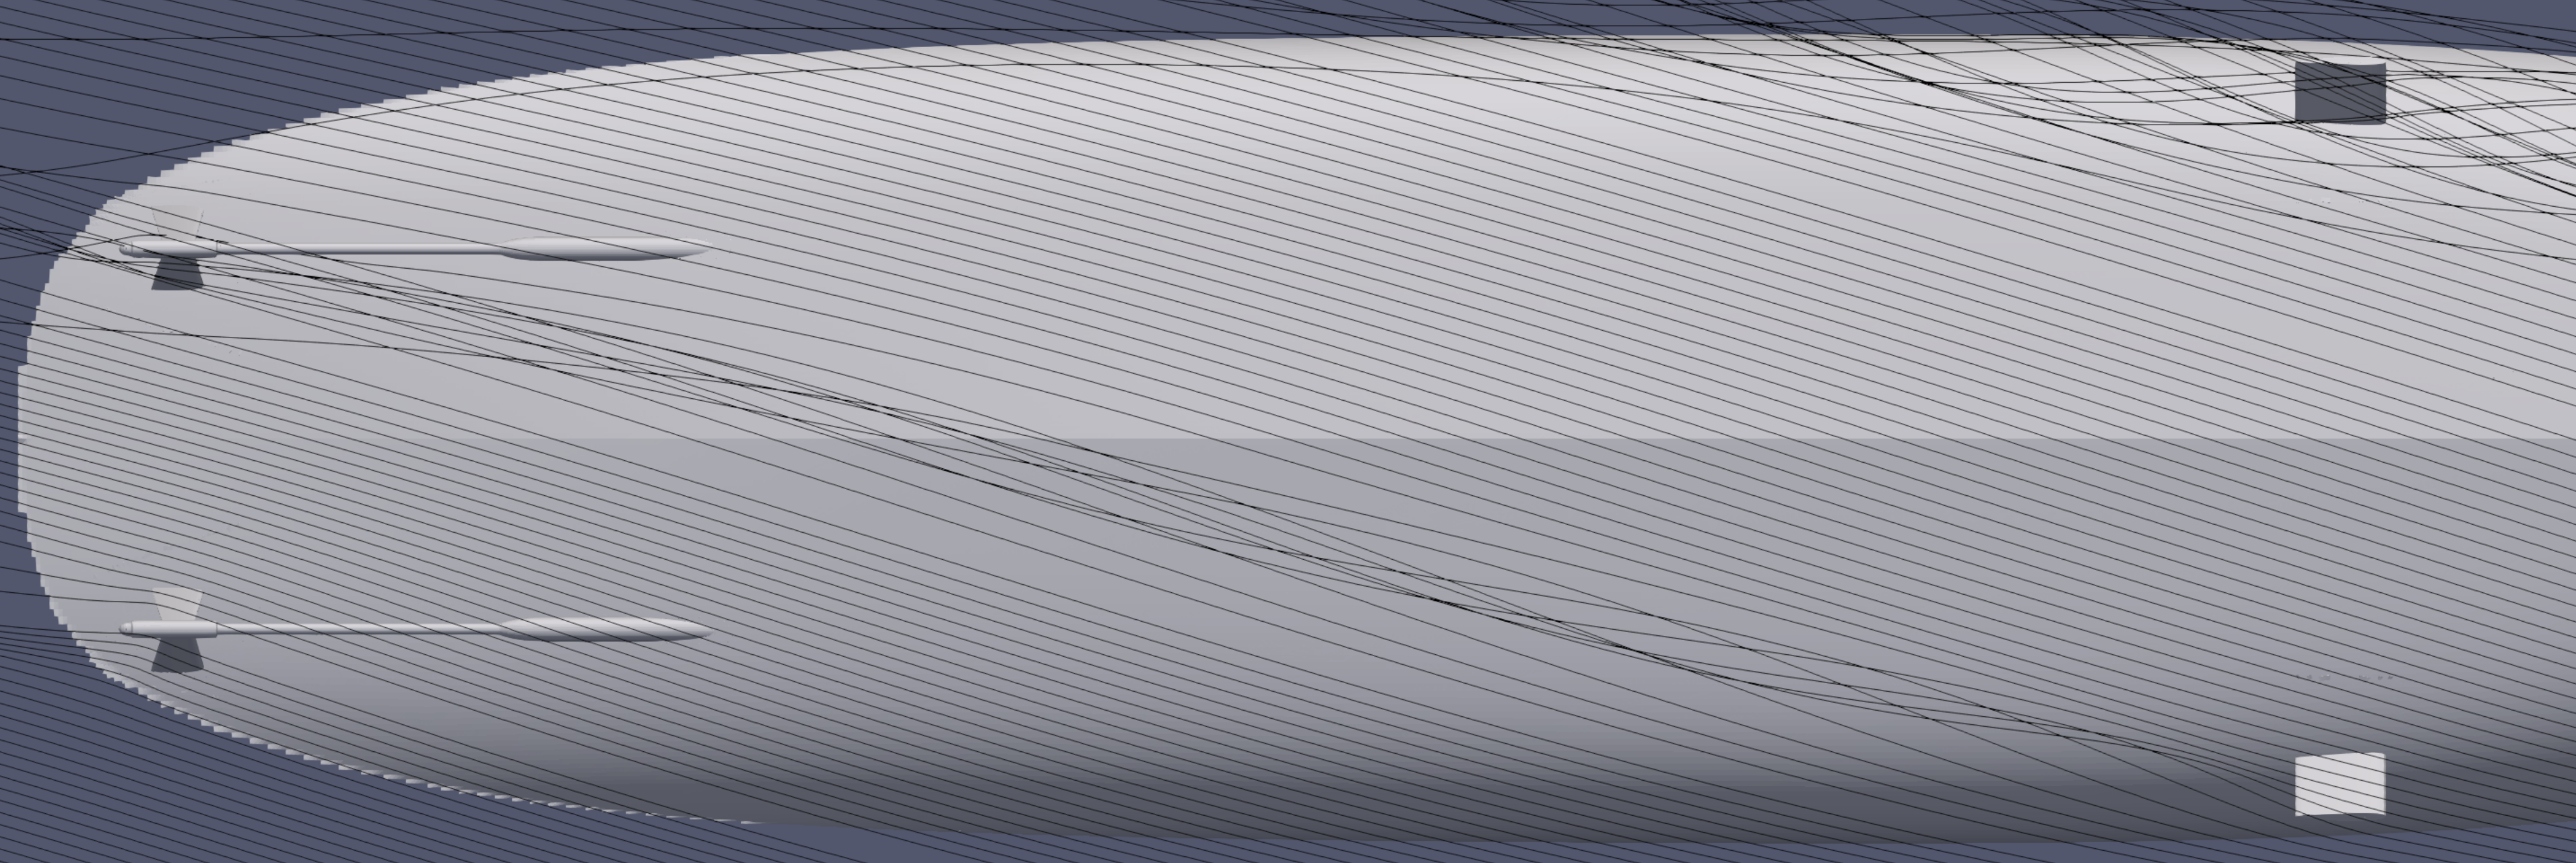
\includegraphics{figures/paraview_drift_15.png}
    \caption{ID estimations of $Y_D$ and $N_D$ during a zigzag20/20 model test compared with model predictions.}
    \label{fig:ID_zigzag20}
\end{figure}